\section{Entity-Relationship Diagramm}

\begin{figure}[ht!]
	\centering{
		\resizebox{0.9\textwidth}{!} {
			\begin{tikzpicture}
				% row by row
				\umlclass[x=18,y=0]{Community}{
					id : Integer \\
					name : String \\
					createdAt : Date \\
					updatedAt : Date
				}{
					PRIMARY(id)
				}

				\umlclass[x=11,y=-6]{User}{
					id: Integer \\
					facebookId: Integer \\
					name: String \\
					createdAt: Date \\
					updatedAt: Date \\
					active: Boolean
				}{
					PRIMARY(id) \\
					UNIQUE(facebookId)
				}

				\umlclass[x=11,y=-13]{Achievement}{
					type: Enum \\
					userId: Integer
				}{
					PRIMARY(type, userId)
				}

				\umlclass[x=18,y=-8]{Task}{
					id: Integer \\
					name: String \\
					description: Text \\
					createdAt: Date \\
					updatedAt: Date \\
					creator: User \\
					fulfillor: User
				}{
					PRIMARY(id)
				}

				\umlclass[x=0,y=-6]{Role}{
					id: Integer \\
					type: Enum\{Resident, \\
						CommunityAdministrator, \\
						Administrator\}
				}{
					PRIMARY(id, type)
				}

				\umlclass[x=5.7,y=-6]{RoleToUser}{
					userId: Integer \\
					roleId: Integer
				}{
					PRIMARY(userId, roleId)
				}

				\umlclass[x=0,y=-10]{Resident}{
					communityId: Integer
				}{}

				% relation
				\umlassoc[mult1=0..*,mult2=1]{Achievement}{User}
				\umlassoc[mult1=1,mult2=0..*]{Community}{Task}
				\umlassoc[mult1=*,mult2=1]{Role}{RoleToUser}
				\umlassoc[mult1=1,mult2=*]{RoleToUser}{User}
				\umlassoc[geometry=-|-, pos2=2.7, mult1=1,mult2=0..*]{User}{Task}
				\umlassoc[geometry=|-|, arm1=-5, anchor1=0.1, pos1=0.5, pos2=2.7,mult1=1,mult2=0..*]{User}{Task}
				\umlassoc[geometry=-|-, mult1=1, mult2=1, pos2=2.98, weight=-0.2]{Resident}{Community}

				% inherit
				\umlinherit[geometry=|-|]{Resident}{Role}
			\end{tikzpicture}
		}
	}

	\caption{Entity-Relationship Diagramm}
\end{figure}